\section{C3PO in Perspective}
As part of this thesis a software prototype is developed that aims to tackle the issues, problems and gaps presented in the previous chapters. The aim is to create a tool that is able to automatically generate a colletion profile of bigger collections (consisting of hundreds of thousands or even millions of objects). 

This profile includes a descriptive statistical representation of the content in the collection, meaning that it contains very specific data such as count of objects, overall size of objects, etc. Furthermore, it provides histogramms of different aspects of the content, such as the file formats, mimetypes, and many other ordinal characteristics that are of interest to the user of the application.

On top of that a service layer enables the user to query the tool in order to gain a deeper insight into the content. This may include the filtering of the content based on different characteristics and splitting it into buckets, which will allow to compare homogeneous parts (based on one or more characteristika) in an otherwise heterogenous content. 

Visualizations and multi dimensional representations of these filterings enable to user to understand the profile and thus provide her with the fundamental knowledge and a more stable ground to take more efficient decisions.
The prototype implementation of the tools is called 'Clever, Crafty Content Profiling of Objects' or c3po for short and is presented in detail in the following subsections.
% idea
% overview
% part of scape, watch source, etc..

\section{Architecture}
In this chapter an overview over the architecture of c3po and its more important aspects are presented.

\subsection{High Level Overview}
C3po is separated into different modules and provides a relatively simple workflow that follows the three steps of content profiling as presented in (TODO cite). In the first part it gathers raw meta data and parses it in order to normalize it into a simple internal data model. In the next step the data is cleaned up, partially aggregated and stored into an external to the tool database.
This offers the baseline for the more deeper analysis provided by some of the modules.


\begin{figure}[htb]
\begin{center}
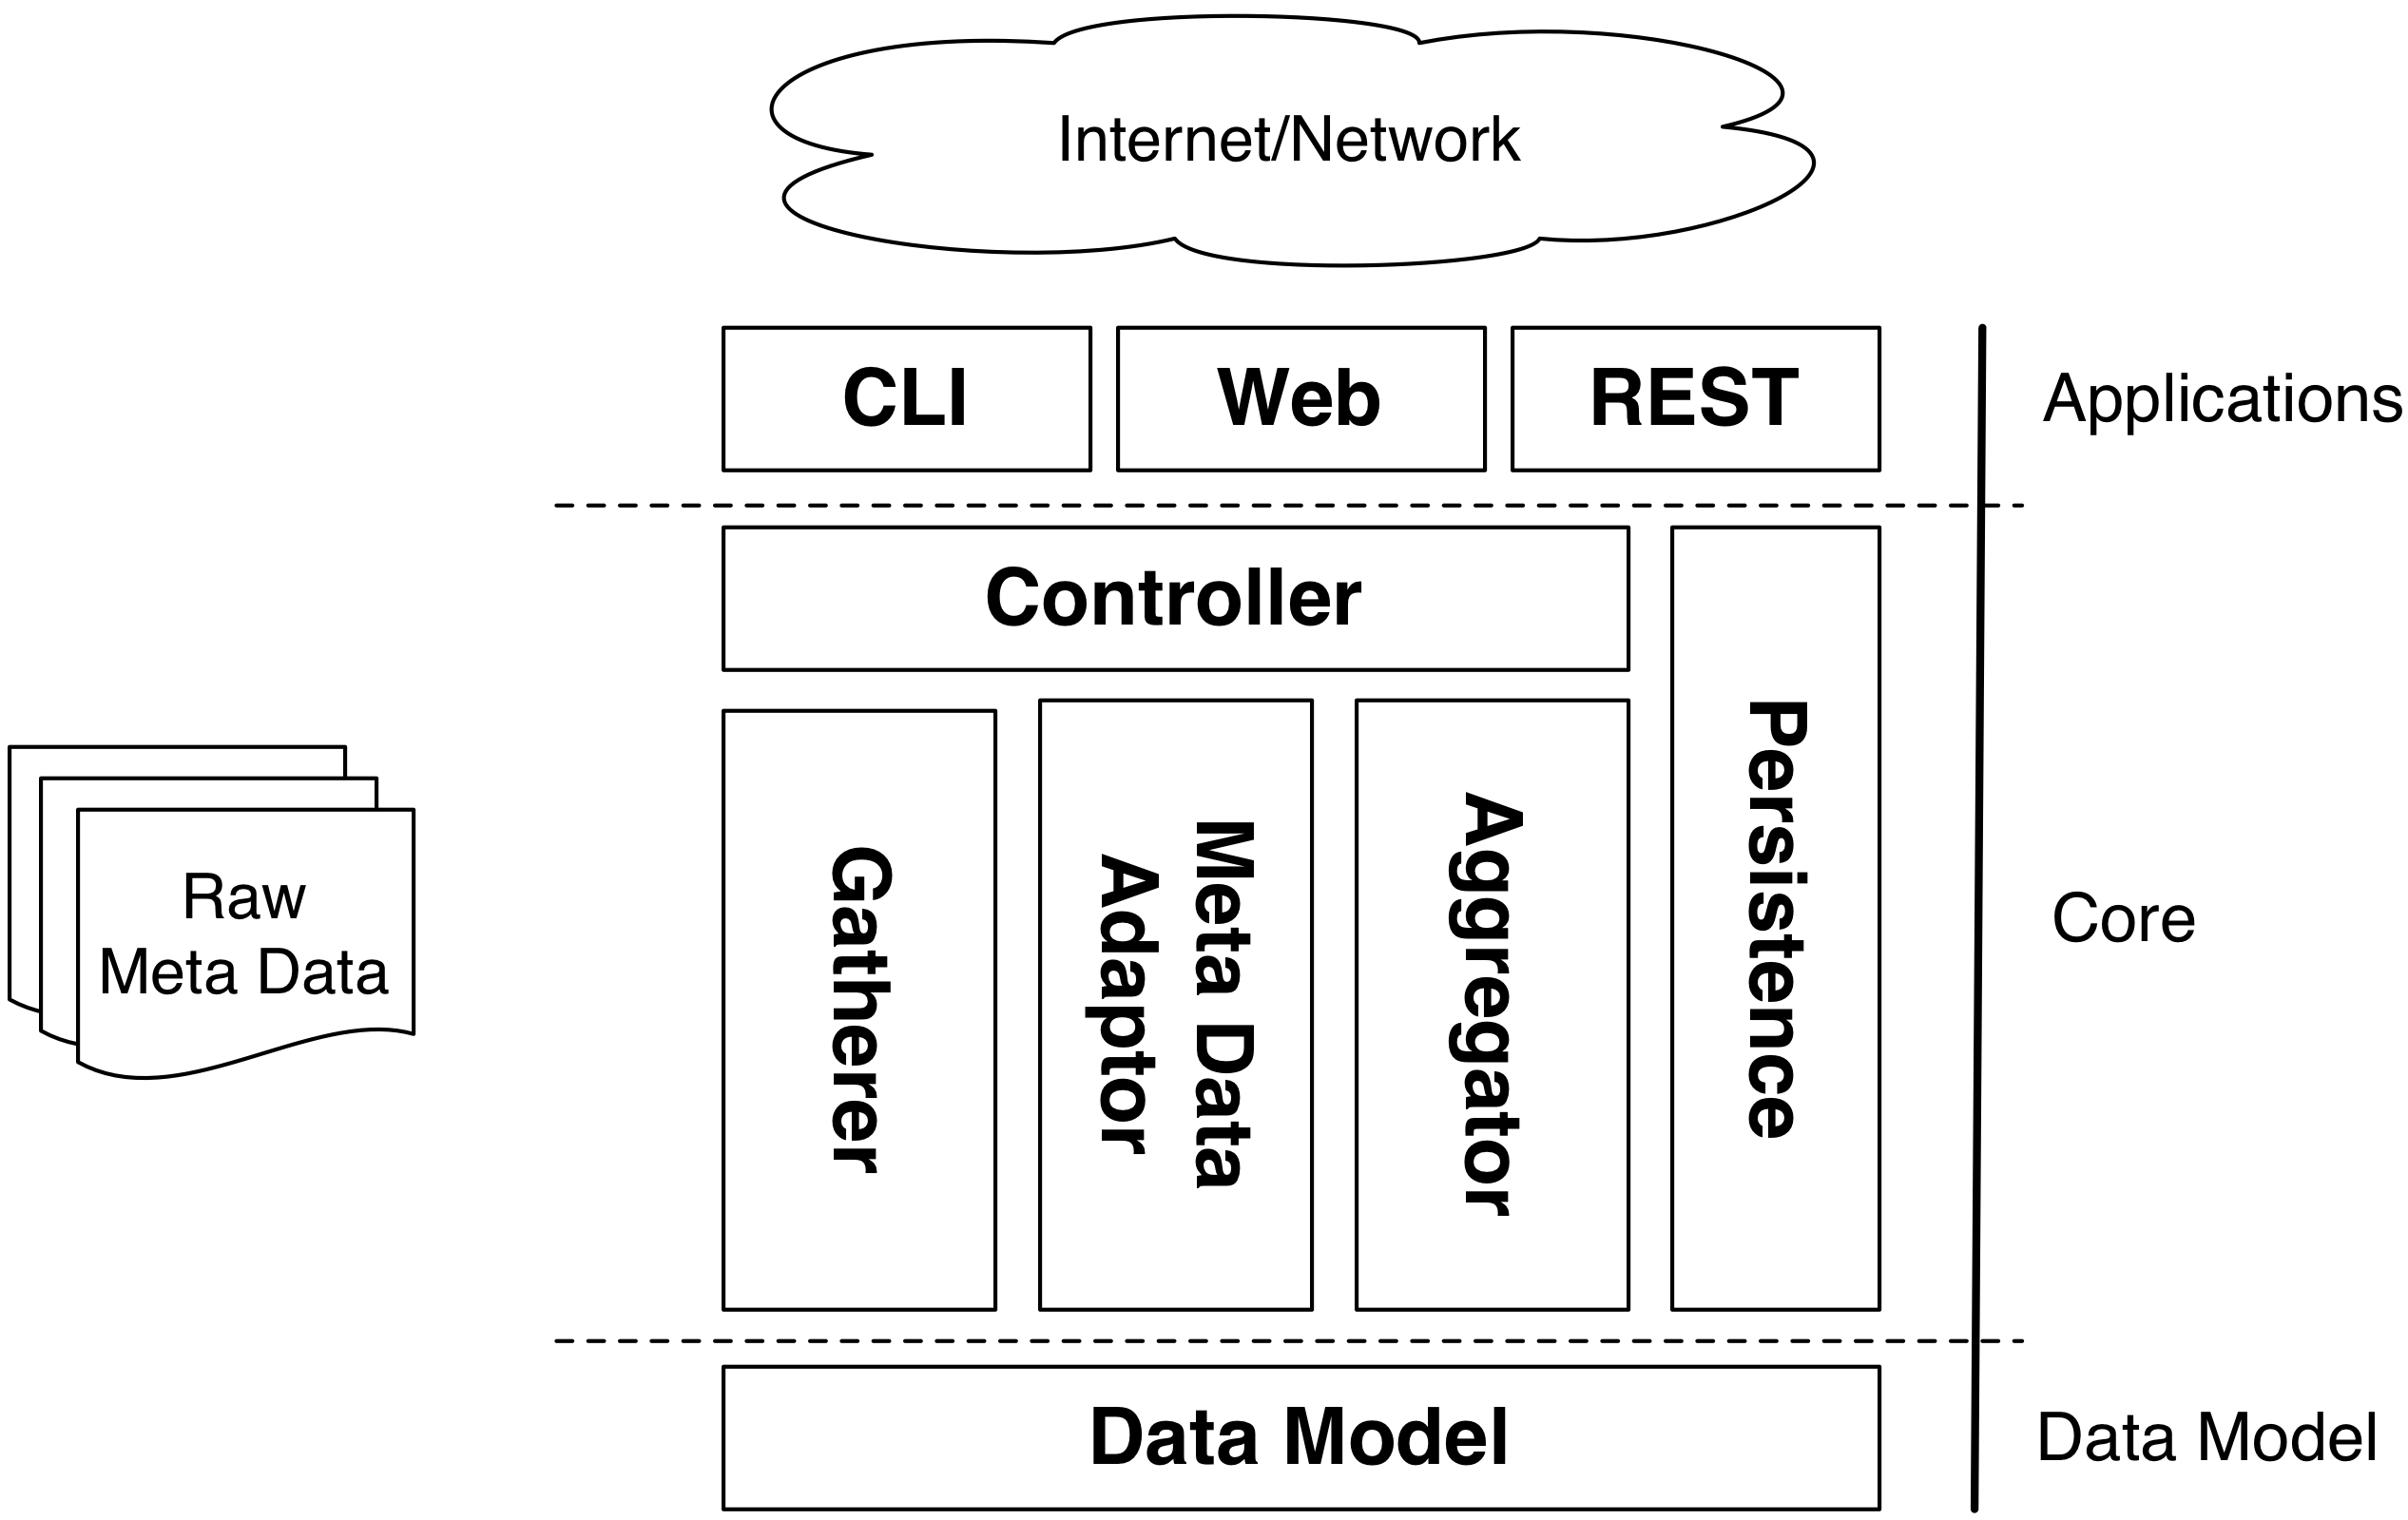
\includegraphics[width=5.5in]{figures/architecture/c3po_highlevel_architecture.png}
\caption{High-level architecture of c3po.}
\label{fig:architecture_highlevel}
\end{center}
\end{figure}

Figure \ref{fig:architecture_highlevel} presents the high level architecture and its modules. At the bottom there is the domain model module which sits as the foundation of the architecture. It represents a simple model able to capture the important aspects of the content meta data in a more generic way but still provides the ability to do flexible queries over the data. It consists mainly of elements - the digital objects and values representing the measurements of specific meta data characteristics. The complete model is provided in (TODO section).

Above that is the main part or the core module, which encapsulates the framework that allows the gathering, normalizing and aggregation of the data. It not only offers interfaces that allow the extension of the framework but also it provides the glue-ware to create and run the work flow.
On top, there is a simple controller, that uses the components below to carry out the work flow. In a first implementation the controller worked in a single threaded, sequential manner due to simplicity reasons. However, preliminary experiments have shown that some tasks, such as meta data parsing make only partial use of the system resources at hand. For example the cpu utilization was mostly less than 25\% during data parsing and storage. Due to this fact the second implementation makes use of a multi-threaded environment which utilizes the available resources much more efficiently. The tool enables the user to configure the number of threads in order to make the most out of the underlying hardware (i.e. hyper-threading).

Below that, there are three important components: the Gatherer, the Meta Data Adaptor and the Aggregator component.
As described in section (TODO cite) the raw meta data of the content can be stored in many different places or sources. For example, it can be provided locally in form of files stored on the local file system, or remotely. The remote source can have many different variations. E.g. there can be a remote ssh server that stores the raw meta data again in file form, or a remote web archive server that stores the meta data in special container files called arc (archive) or warc (web archive) file, but there can be also a remote repository, which not only stores the original content but all the meta data for each object in a different way (internal data store, to its local file system, etc.). The latter represents the most likely use case in a real world digital preservation scenario, however all others are possible as well, not to mention that they are easier to use for experimentation purposes.

As the users of c3po should not be interested in the way of how and where the meta data is stored, the gatherer component offers an interface, which provides an abstraction to all these differences and exposes a unified interface allowing the Controller to obtain streams to the next N files that have to be processed. This design allows a transparent view to the other modules in the system. c3po provides an implementation only for local file systems, however extending the tool to be able to fetch data from a different source is just a matter of implementing a single interface, which is able to count the files to be processed and to open streams to the next N files. It is up to the implementing class to decide whether the data will be retrieved over the network and the stream will be passed directly for further processing or it will be cached in batches to the local file system. Depending on the use case both could make sense and thus it is left in the responsibility of the service provider.
%Eventually, say that there is no restriction currently of how the implementation shall look like, e.g. direct stream over the network or  temporary storage to the local system.

Since different sources can use different characterization tools and different characterization tool outputs, the Meta Data Adaptor component is responsible for instantiating and assigning a specific implementation of an adaptor that can handle the gathered meta data records. Each meta data adaptor runs in a thread and is responsible for parsing meta data files that conform to a specific meta data schema. The c3po protoype makes use of a single adaptor for the FITS output format as described in (TODO cite). Extending to other formats is straight forward and a matter of another interface implementation.

% TODO implement and describe aggregator.

The last part of the core module is the persistence layer.
In a first iteration c3po's persistence layer was based on the Java Persistence API\footnote{http://docs.oracle.com/javaee/6/tutorial/doc/bnbpz.html} (JPA 1.0) with Hibernate\footnote{http://www.hibernate.org/} as the persistence provider. The higher level abstraction was done via a couple of generic data access object (DAO) interfaces, which were implemented by the client application, and client modules.

This design was chosen in order to allow each client application to choose its own implementation of the persistence layer. This was important since c3po is meant to be deployable in application server containers, so that queries by other tools and users can be done over the network. For this, a special container managed transactional model would be needed. On the other hand, content profiling is a data intensive process, which can gain from the fact that the tool can execute near the data. That is why, also a local transactional model is needed, in which the tool is run locally near the data without any application server. All this allows the separation of the data gathering and the data analysis parts of the work flow. The fact that the data base is external to the tool also means that it can be setup near the data or on a specific storage sever that has enough resources at its hand to handle the load.

There is a command line application that offers an implementation of c3po persistence layer apis/daos and also there is the web module, which has a container managed implementation. The web module represents the last part of the tool, where a simple web application that exposes some of the functionality of the tool over a REST \cite{Fielding:2000:ASD:932295} interface. REST was chosen for two main reasons. For one, it is easy to understand and pretty straightforward to implement. This allows easy integration with other tools, such as monitoring services (TODO cite) and a variety of client applications. The second reason is that other technologies, such as JavaServer Faces Technology\footnote{http://www.oracle.com/technetwork/java/javaee/javaserverfaces-139869.html} (JSF) and Enterprise Java Beans Technology\footnote{http://www.oracle.com/technetwork/java/javaee/ejb/index.html} (EJB) would have meant that only a few application servers will be compliant and able to support the application. As already mentioned, easy deployment is part of the requirements and thus the implementation shall avoid relying on frameworks that are restricting the choice of the server.
%REST cite: http://www.ics.uci.edu/~fielding/pubs/dissertation/rest_arch_style.htm

However, after the first iteration this implementation has proven to be infeasible. From a design point of view, everything seemed to be clean and the separation of concerns allowed each client to use its own implementation. However, the relational paradigm and the ORM mapper proved to be a significant bottleneck. On the one hand the overhead of the ORM mapper was proven to be unnecessary during meta data adaptation and storage. On the other hand the analysis of the data seemed to take a unnecessary long time due to the many joins. One could argue that the joins could have been avoided by making the data model more specific, however this would have comprimised the flexibility which was a huge trade off.
For these two reasons the data model was analysed again and different storage possibilities were evaluated. 
Due to the natural key-value structure of the meta data it seemed that a key value store would possibly provide better solution to the problem. However, usually key-value stores are used for caching (ECache, Memchahe, etc.) and architecutre designers often have problems fitting their datamodel when such technologies are used for more than their purpose - caching.
There are some implementations of data bases that offer most of the flexibility of the relational paradigm, high performance due to their almost key-value paradigm and out of the box horizontal scalability. 
MongoDB\footnote{http://www.mongodb.org/} is a document store that uses BSON\footnote{http://bsonspec.org/} (Binary JSON) in order to store documents. These documents can have any kind of structure and do not have to be normalized in the relational database sense. On top of that MongoDB provides native facilities for executing Map Reduce \cite{Dean:2008:MSD:1327452.1327492} jobs on the server, which were proven to be very useful for aggregating and filtering the data.
The second iteration provided such a backend that uses a Mongo document store. Preliminary test results have shown that parsing the meta data and storing it for a collection of about ~550 thousand files was done in about 17 minutes on a laptop, whereas the old solution needed about 12 hours for the same set of files on the same machine.
Furthermore, exporting a sparse matrix of all property values for every element in the collection was proven to be much faster. This was due to the fact, that the internal representation of the data needed no JOINS anymore and can be done by single iteration over a database cursor.

\subsection{Data Model}
This section gives an overview of the current datamodel and why it was chosen as well as a short overview of the first model used.
\subsubsection{Relational Data Model}
As relational databases have stood the test of time and are proven to work in virtually any use case, the natural thing was to try a relational model first.
Figure \ref{fig:old_datamodel} shows a simplified version of the key domains of the first data model used. It models the key concepts for generic key value structure in a relational database, which would fit the needs of the collection profiler and leaves out some fields and helper classes. 

The \textit{Elements} describe the objects. Each element has a number of \textit{Values}, where every value is a measurement for a specific \textit{Property}. Properties are specific charactersistics, such as format, size, or nr of pages in a document. 

There are different typed values for the different data types, such as String, Bool, Numeric, Float and Array, which are not shown in the diagram. Furthermore, each value has a \textit{ValueSource}, which provides provenance information.

Although this model was so minimalistic it was proven to be uncapable of a high enough performance when querying more specific information (a mixture of more properties and values) due to the generic nature of the Values. One special requirement was the query/export of a sparse matrix over a number of properties for each element. This use case provides the user with a great overview of the data and enables her to find important aspects that would otherwise easily evade. Since the data is sparse it was not feasible to query the described matrix of the data in an efficient way, which made the implementation of this key requirement hard.

The underlying data store was a PostgreSQL, which is one of the best open relational databases at the time of writing. However, the limitation of the high number of JOINS for the sparse matrix use case is just contradictory to the paradigm, since there is a general rule of thumb that more JOINS result in a poor performance. Through data model enhancements and optimizations and a lot of query optimization it probably would have been possible to use a relational model effectively. However, this was not the focus of the work, so a new approach was chosen.

\begin{figure}[htb]
\begin{center}
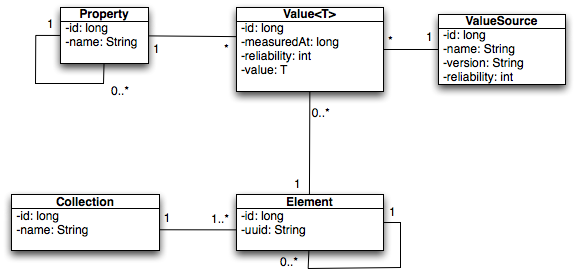
\includegraphics[width=5in]{figures/architecture/old_datamodel.png}
\caption{Old datamodel used in the first iteration.}
\label{fig:old_datamodel}
\end{center}
\end{figure}

\subsubsection{Document Store Schema}
After examination of the data at hand it seemed that the key value structure was fitting, but through the normalization, performance was compromized. A MongoDB document store schema was chosen for a number of reasons:
\begin{itemize}
\item Natural fit of the data into a key-value schema
\item Native Map-Reduce support for data aggregation
\item Query cursor and pagination
\item Horizontal scaling and automatic node balancing out of the box
\end{itemize}

There are three main collections (here the term collection is used in the sense of a document store and can be understood as the equivalent concept of a table in a relational database). One for the elements, one for the properties and one for the sources. The values are embedded into each element document and thus each document represents a self-contained object with all its known meta data - values, sources and conflicts. This has one big advantage when querying as all values are already there whithout a need of joining the property table. Furthermore the equivalent of a SELECT statement in MongoDB does not retrieve the actual data, but only a cursor over it.
Figure \ref{fig:document_structure} gives an orveview of the basic structure of element documents in BSON syntax. Note that the syntax is very similar to JSON, but provides data type support (e.g. the ObjectId).

\begin{figure}[htb]
\begin{center}
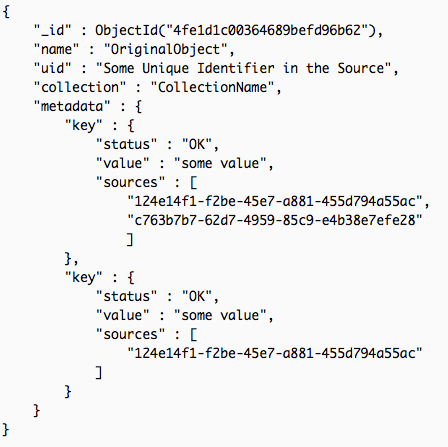
\includegraphics[width=4in]{figures/architecture/document_structure.png}
\caption{Structure of a c3po element in BSON.}
\label{fig:document_structure}
\end{center}
\end{figure}

Since Map-Reduce jobs are supported natively in MongoDB, it is easy to do simple aggregation over some specific value of a specific key in every element document. Another great advantage of this implementation is the pagination support. Every query in Mongo DB returns a cursor over the data rather then the data itself. This makes navigation over the data within an application fast and efficient in terms of memory, as one does not have to consider the volume of the queried data.
The third reason, why Mongo was chosen, was the automatic load balancing used by the document store server. The document store supports horizontal scaling and auto node balancing out of the box, which might turn up useful when considering the amounts of data that the profiler has to deal with.

\subsection{Interfaces and Extension Points}

\subsection{Web Application}
The Web Application is written using the PlayFramework\footnote{http://www.playframework.org/} for the backend and the API and standard HTML5 and Javascript for the front end user interface. It enables the user to
select her collection and obtain deeper overview by filtering the data based on specific properties and values as shown in figure \ref{fig:web_app_overview}.

\begin{figure}[htb]
\begin{center}
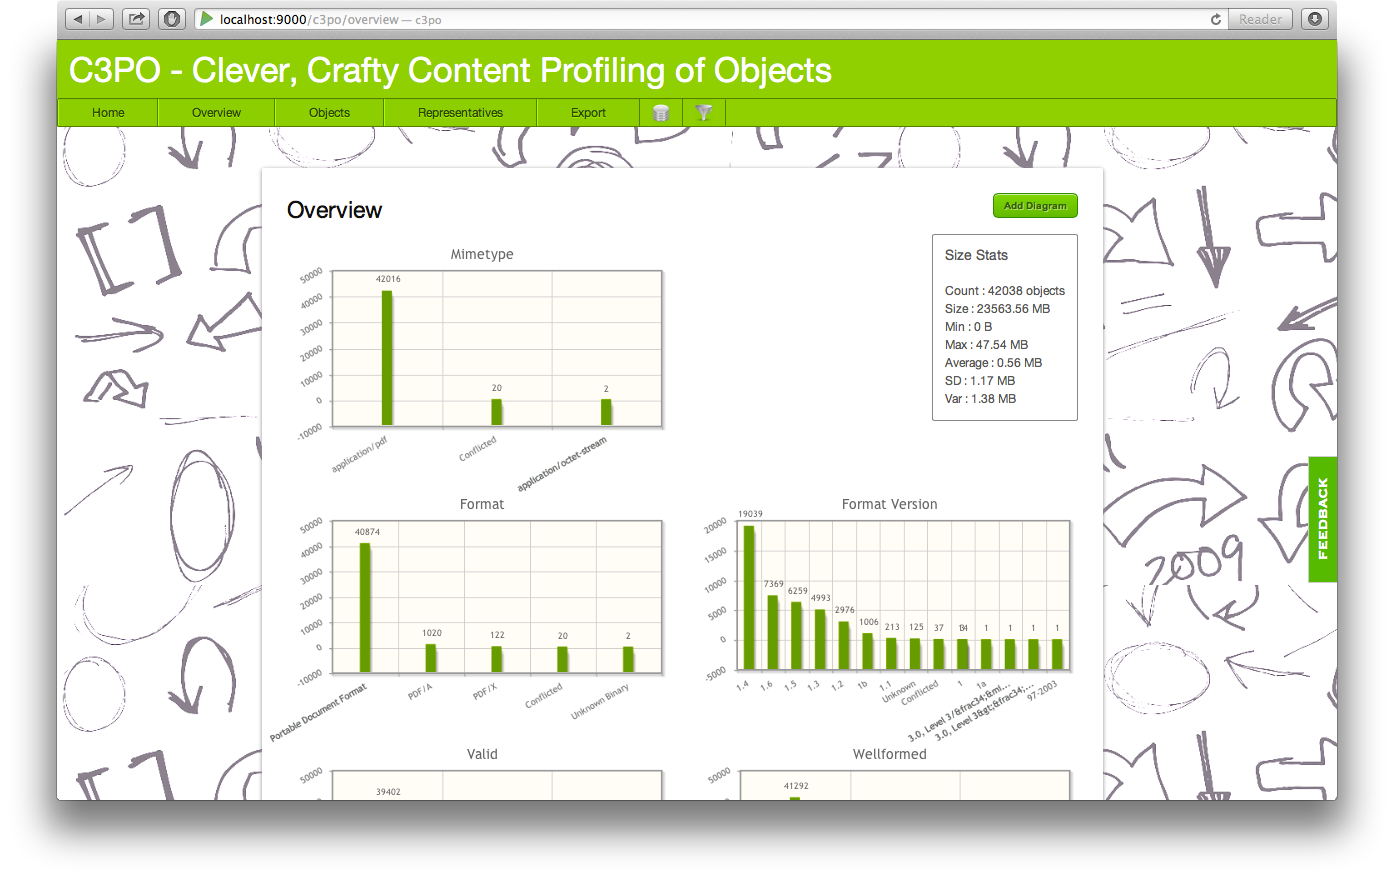
\includegraphics[width=5.5in]{figures/architecture/web_app_overview}
\caption{Screenshot of c3po - part of the overview of a collection.}
\label{fig:web_app_overview}
\end{center}
\end{figure}


\subsection{Build Process and Deployment}
The separation of the high level architecture into modules is not only done in a logical fashion. By using a widely spread and used build management tool called Maven\footnote{http://maven.apache.org} the code is separated into different packages, that can be found at \url{http://github.com/peshkira/c3po}. Maven is responsible for fetching and managing all the dependencies and their correct versions for c3po.
All this makes the distribution and maintainability of the application much easier as well as it provides an easy build process.

\section{Representative Sets}

\section{Future Points of Interest}
There are many topics that can be handled and implemented in future work. Here we outline some and briefly discuss them:
\begin {itemize}
\item \textit{Scalability} is very important as the volumes of data will grow more and more over time. Even though the hardware resources and provided performance also grow over time the issue of scalability is very important. The authors believe that horizontal scalability is the best way to pursue. The current design decisions follow that path. More specifically, future enhancements should include the distributed map-reduce jobs and the caching of specific results, which will enhance the systems responsiveness.
\item \textit{Continous Profiling} is important as collections change over time. The support for including meta data of new and changed objects as well as adapting the computed aggregations in a easy, fast and scalable fashion is critical for the success of such an application in productuin use. Thus the investigation of the problems that arise with this will be important for future versions of the tool. The Map-Reduce facilities provide a potential solution to such a problem, since it is possible to aggregate new data and reuse old results, which are then just merged as the reduce function is always the same. 
\item \textit{Input to Digital Preservation Tools}. Monitoring systems and Simulators enhance the preservation planning processes by providing relevant and trustworthy information that is often hard to obtain due to its distribution and by offering simulations and projections of different outcomes based on current decisions and policies. Such systems heavily rely on larger amount of data. An integration with a content profile tool will play an important role for such tools as well as preservation planning activities.
\item \textit{Representative Sets} are the foundation for unbiased experiments and thus better performing algorithms in terms of speed and effective slection should be the focus of future work as well. 
\end{itemize}

